The density of states plays a significant role in understanding electronic band
structure in solid state physics, and so several methods have been proposed in
that literature to estimate spectral densities. We review two such methods: the
kernel polynomial method (KPM) which involves a polynomial expansion of the
DOS/LDOS, and the Gauss Quadrature via Lanczos iteration (GQL). These methods
have not previously been applied in the network setting, though Cohen-Steiner et
al.~\cite{cohen2018approximating} have independently invented an approach
similar to KPM for the global DOS alone, albeit using a less numerically stable
polynomial basis (the power basis associated with random walks). We then
introduce a new direct nested dissection method for LDOS, as well as new
graph-specific modifications to improve the convergence of the KPM and GQL
approaches.

Throughout this section, $H$ denotes any symmetric matrix.

\subsection{Kernel Polynomial Method (KPM)}\label{subsec:kpm}

The Kernel Polynomial Method (KPM)~\cite{weisse2006kernel} approximates the
spectral density through an expansion in the dual basis of an orthogonal
polynomial basis. Traditionally, the Chebyshev basis $\{T_m\}$ is used because
of its connection to the best polynomial interpolation. Chebyshev approximation
requires the spectrum to be supported on the interval $[-1,1]$ for numerical
stability. However, this condition can be satisfied by any graph matrix after
shifting and rescaling:
\begin{equation}\label{eqn:shiftscale}
	\widetilde{H} = \frac{2H - (\lambda_{\max}(H)+\lambda_{\min}(H))}{\lambda_
	{\max}(H) - \lambda_{\min}(H)}\,.
\end{equation}
We can compute these extremal eigenvalues efficiently for our sparse matrix $H$,
so the pre-computation is not an issue~\cite{Parlett-1984-sparse}.

As defined in \cref{eqn:cheb_3term}, the Chebyshev polynomials $T_m(x)$ satisfy
the recurrence
\begin{equation*}
	T_0(x) = 1,\; T_1(x) = x,\; T_{m+1}(x) = 2xT_m(x) - T_{m-1}(x)\,.
\end{equation*}
They are orthogonal with respect to $w(x) =  2 / \left[(1+\delta_{0n})\pi
\sqrt{1-x^2}\right]$:
\begin{equation} \label{eqn:orth}
	\int_{-1}^1 w(x)T_m(x)T_n(x)dx = \delta_{mn}\,.
\end{equation}
(Here and elsewhere, $\delta_{ij}$ is the Kronecker delta: $1$ if $i = j$ and
$0$ otherwise.) Therefore, $T_m^\ast(x) = w(x)T_m(x)$ also forms the dual
Chebyshev basis. Using Eq. \ref{eqn:orth}, we can expand our DOS $\mu(\lambda)$
as
\begin{gather} \label{eqn:doscoeff}
\mu(\lambda) = \sum_{m=0}^\infty d_mT^\ast_m(\lambda)\,, \\
d_m = \int_{-1}^1T_m(\lambda)\mu(\lambda)d\lambda = \frac{1}{N}\sum_{i=1}^N 
T_m(\lambda_i) = \frac{1}{N}\tr(T_m(H))\,.
\end{gather}
Here, $T_m(H)$ is the $m$\hyp{}th Chebyshev polynomial of the matrix $H$. The
last equality comes from the spectral mapping theorem, which says that taking a
polynomial of $H$ maps the eigenvalues by the same polynomial. Similarly, we
express the PDOS $\mu_k(\lambda)$ as
\begin{equation}\label{eqn:pdoscoeff}
	d_{mk} = \int_{-1}^1 T_m(\lambda)\mu_k(\lambda)d\lambda = \sum_{i=1}^N |q_i(k)|
	^2T_m(\lambda_i) = T_m(H)_{kk}\,.
\end{equation}

We want to efficiently extract the diagonal elements of the matrices $\{T_m
(H)\}$ without forming them explicitly; the key idea is to apply the stochastic
trace/diagonal estimation, proposed by Hutchinson~
\cite{hutchinson1990stochastic} and Bekas et al.~\cite{bekas2007estimator}.
% Given a random probe vector $z$ such that $z_i$'s are i.i.d.~with mean $0$ and
% variance $1$,
% \begin{equation}\label{eq:probe_trace}
% 	\BBE[z^THz] = \sum_{i,j}H_{ij}\BBE[z_iz_j] = \tr(H)
% \end{equation}
% \begin{equation}\label{eq:probe_diag}
% 	\BBE[z\odot Hz] = \diag(H)
% \end{equation}
% where $\odot$ represents the Hadamard (elementwise) product. Choosing $N_z$
% independent probe vectors $Z_j$, we obtain the unbiased estimator
% \begin{equation}
% 	\tr(H) = \BBE[z^THz] \approx \frac{1}{N_z}\sum_{j=1}^{N_z}Z_j^THZ_j 
% \end{equation}
% and similarly for the diagonal. \citet{avron2011randomized} review many possible
% choices of probes for \cref{eq:probe_trace,eq:probe_diag}; a common choice is
% vectors with independent standard normal entries. 
We have described the details in \cref{pre:ste}. Using the Chebyshev recurrence 
(\cref{eqn:cheb_3term}), we can compute the sequence $T_m(H)z$ for each probe at
a cost of one matrix-vector product per term, for a total cost of $\calO(
\abs{E}N_z)$ time per moment $T_m(H)$.
\begin{equation}\label{eqn:3term_vec}
	T_{m+1}(H)z = 2HT_m(H)z - T_{m-1}(H)z\,.
\end{equation}

In practice, we only use a finite number of moments rather than an infinite
expansion. The number of moments required depends on the convergence rate of the
Chebyshev approximation for the class of functions DOS/LDOS is integrated with.
For example, the approximation error decays exponentially for test functions
that are smooth over the spectrum \cite{Trefethen-2013-ATAP}, so only a few
moments are needed. On the other hand, such truncation leads to Gibbs
oscillations that cause error in the interpolation ~\cite{Trefethen-2013-ATAP}.
However, to a large extent, we can use smoothing techniques such as Jackson
damping to resolve this issue ~\cite{jackson1911genauigkeit} (we will formalize
this in \cref{thm:Jackson_damping}).

\subsection{Gauss Quadrature and Lanczos (GQL)}

This method builds of the Gauss Quadrature and Lanczos (GQL) algorithm we
introduced in \cref{pre:fom}. Using the same stochastic estimation from 
\cref{subsec:kpm}, we can also apply GQL to compute DOS.

% Golub and Meurant developed the well-known Gauss Quadrature and Lanczos (GQL)
% algorithm to approximate bilinear forms for smooth functions of a matrix~
% \cite{golub1997matrices}.  Using the same stochastic estimation from \S~
% \ref{subsec:kpm}, we can also apply GQL to compute DOS.

For a starting vector $z$ and graph matrix $H$, Lanczos iterations after
$M$ steps produce a decomposition
\begin{equation*}
	HZ_M = Z_M\Gamma_M + r_Me_M^T\,,
\end{equation*}
where $Z_M^TZ_M = I_M$, $Z_M^Tr_M = 0$, and $\Gamma_M$ tridiagonal. GQL
approximates $z^Tf(H)z$ with $\norm{z}^2e_1^Tf(T_M)e_1$, implying
\begin{equation}
	z^Tf(H)z = \sum_{i=1}^N \abs{z^Tq_i}^2f(\lambda_i) \approx \norm{z}^2\sum_
	{i=1}^M\abs{p_{i1}}^2f(\tau_i)\,,
\end{equation}
where $(\tau_1,p_1)\cdots,(\tau_M, p_M)$ are the eigenpairs of $\Gamma_M$. 
Consequently,
\begin{equation}
	\norm{z}^2\sum_{i=1}^M \abs{p_{i1}}^2\delta(\lambda-\tau_i)
\end{equation}
approximates the LDOS $\mu(\lambda; z)$.

Building upon the stochastic estimation idea and the invariance of probe 
vectors under orthogonal transformation, we have
\begin{equation}
	\BBE[\mu(\lambda;z)] = \sum_{i=1}^N \delta(\lambda-\lambda_i) = N\mu
	(\lambda)\,.
\end{equation}
Hence 
\begin{equation}
	\mu(\lambda)\approx\sum_{i=1}^M |p_{i1}|^2\delta(\lambda-\tau_i)\,.
\end{equation}
The approximate generalized function is exact when applied to polynomials of
degree $\Leq 2M+1$. Furthermore, if we let $z = e_k$ then GQL also provides an
estimation for the PDOS $\mu_k(\lambda)$. Estimation from GQL can also be
converted to Chebyshev moments if needed.

\subsection{Nested Dissection (ND)}

The estimation error via Monte Carlo method intrinsically decays at the rate
$\calO(1 /\!\!\sqrt{N_z})$, where $N_z$ is the number of random probing vectors.
Hence, we have to tolerate the higher variance when increasing the number of
probe vectors becomes too expensive. This is particularly problematic when we
try to compute the PDOS for all nodes using the stochastic diagonal estimator.
Therefore, we introduce an alternative divide-and-conquer  method, which
computes more accurate PDOS for any set of nodes at a cost comparable to the
stochastic approach in practice.

Suppose the graph can be partitioned into two subgraphs by removal of a small
vertex separator.  Permuting the vertices so that the two partitions appear
first, followed by the separator vertices. Up to vertex permutations, we can
rewrite $H$ in block form as
\begin{equation}\label{eqn:dissection}
	H = \begin{bmatrix}
	H_{11} & 0 & H_{13}\\
	0 & H_{22} & H_{23}\\
	H_{13}^T & H_{23}^T & H_{33}
	\end{bmatrix},
\end{equation}
where the indices indicate the groups identities. Leveraging this structure, we
can update the recurrence relation for Chebyshev polynomials to become
\begin{equation}\label{eqn:ndcheb}
	T_{m+1}(H)_{11} = 2H_{11}T_m(H)_{11} - T_{m-1}(H)_{11} + 2H_{13}T_m(H)_{31}\,.
\end{equation}

Recursing on the partitioning will lead to a nested dissection, after which we
will use direct computation on sufficiently small sub-blocks. We denote the
indexing of each partition with $I^{(t)}_p = I^{(t)}_s\bigcup I^{
(t)}_\ell\bigcup I^{(t)}_r$, which represents all nodes in the current
partition, the separators, and two sub-partitions, respectively. For the
separators, \cref{eqn:ndcheb} leads to
\begin{align}\label{eqn:ndchebsep}
	&T_{m+1}(H)(I^{(t)}_p,I^{(t)}_s) = 2H(I^{(t)}_p, I^{(t)}_p)T_m(H)(I^{(t)}_p,
	I^{(t)}_s) \nonumber\\
	&-T_{m-1}(H)(I^{(t)}_p,I^{(t)}_s) + 2\sum_{t'\in S_t}H(I^{(t)}_p,I^{(t')}_s)
	T_m(H)(I^{(t')}_s, I^{(t)}_s)\,,
\end{align}
where $S_t$ is the path from partition $t$ to the root; and for the leaf
blocks, $I^{(t)}_s = I^{(t)}_p$ in \cref{eqn:ndchebsep}. The result is 
\cref{alg:ndpdos}.

\begin{algorithm}
	\SetKwInput{KwInput}{Input}
	\SetKwInput{KwOutput}{Output}
	\DontPrintSemicolon
		\KwInput{Symmetric graph matrix $H$ with eigenvalues in $[-1,1]$}
		\KwOutput{$C\in\BBR^{N\times M}$ where $c_{ij}$ is the $j$-th Chebyshev
		moment for $i$-th node.}
		\Begin{
			Obtain partitions $\{I^{(t)}_p\}$ in a tree structure through
			multilevel nested dissection.\;
			\For{$m=1$ \textbf{to} $M$}{
				Traverse partition tree in pre-order:\;
				\quad Compute the separator columns with \cref{eqn:ndchebsep}.\;
				\quad \If{$I^{(t)}_p$ is a leaf block}{Compute the diagonal entries
				with equation (\ref{eqn:ndchebsep}).}
			}
		}
	\caption{Nested Dissection for PDOS Approximation}
	\label{alg:ndpdos}        
\end{algorithm}

The multilevel nested dissection process itself has a well-established
algorithm by \citeauthor{karypis1998fast}, and efficient implementation is
available in \texttt{METIS}~\cite{karypis1998fast}. Note that this approach is
only viable when the graph can be partitioned with a separator of small size.
Empirically, we observe this assumption to hold for many real-world networks.
The biggest advantage of this approach is we can very efficiently obtain PDOS
estimation for a subset of nodes with much better accuracy than KPM.


\subsection{Motif Filtering}

In many graphs, there are large spikes around particular eigenvalues; for
example, see \cref{fig:caida}. This phenomenon affects the accuracy of DOS
estimation in two ways. First, the singularity-like behavior means we need many
more moments to obtain a good approximation in polynomial basis. Secondly, due
to the equi-oscillation property of Chebyshev approximation, error in
irregularities (say, at a point of high concentration in the spectral density),
spreads to other parts of the spectrum. This is a problem in our case, as the
spectral density of real-world networks are far from uniform.

High multiplicity eigenvalues are typically related to local symmetries in a
graph. The most prevalent example is two dangling nodes attached to the same
neighbor as shown in \cref{fig:motif_0}, which accounts for most eigenvalues
around $0$ for (normalized) adjacency matrix with a localized eigenvector taking
value $+1$ on one node and $-1$ on the other. In addition, we list a few more
motifs in \cref{fig:motifs} that appear most frequently in real-world graphs.
All of them can be associated with specific eigenvalues, and we include the
corresponding ones in normalized adjacency matrix for our example.

\begin{figure}[htp]
	\begin{center}
  \begin{subfigure}{\textwidth}
  	\centering
		\begin{tikzpicture}[remember picture, overlay]
			\node[draw,line width=1mm,circle,inner sep=1mm] (A) at (-4,0) 
			{${\color{blue}\bm{+1}}$};
			\node[draw,line width=1mm,circle,inner sep=1mm] (B) at (-2,0)
			{${\color{red}\bm{-1}}$};
			\node[draw,line width=1mm,fill=gray,circle,inner sep=3mm] (C) at 
			(-3,-1) {};
			\node[draw,line width=1mm,circle,inner sep=1mm] (D) at (1,0)
			{${\color{red}\bm{-1}}$};
			\node[draw,line width=1mm,circle,inner sep=1mm] (E) at (3,0)
			{${\color{blue}\bm{+1}}$};
			\node[draw,line width=1mm,circle,inner sep=1mm] (F) at (5,0)
			{${\color{red}\bm{-1}}$};
			\node[draw,line width=1mm,fill=gray,circle,inner sep=3mm] (G) at 
			(2,-1) {};
			\node[draw,line width=1mm,fill=gray,circle,inner sep=3mm] (H) at 
			(4,-1) {};

			\draw[line width=1mm] (A)--(C);
			\draw[line width=1mm] (B)--(C);
			\draw[line width=1mm, loosely dashed] (-4.5,-2)--(C);
			\draw[line width=1mm, loosely dashed] (-1.5,-2)--(C);
			\draw[line width=1mm] (D)--(G);
			\draw[line width=1mm] (E)--(G);
			\draw[line width=1mm] (E)--(H);
			\draw[line width=1mm] (F)--(H);
			\draw[line width=1mm, loosely dashed] (.5,-2)--(G);
			\draw[line width=1mm, loosely dashed] (3.5,-2)--(G);
			\draw[line width=1mm, loosely dashed] (2.5,-2)--(H);
			\draw[line width=1mm, loosely dashed] (5.5,-2)--(H);
		\end{tikzpicture}
		\vspace{2.5cm}
		\caption{$\lambda=0$}\label{fig:motif_0}
	\end{subfigure}
  %
  \begin{subfigure}{\textwidth}
  	\centering
		\begin{tikzpicture}[remember picture, overlay]
			\node[draw,line width=1mm,circle,inner sep=1mm] (A) at (-5,-1) 
			{${\color{blue}\bm{+1}}$};
			\node[draw,line width=1mm,circle,inner sep=1mm] (B) at (-3.75,-1)
			{${\color{green}\bm{\pm 1}}$};
			\node[draw,line width=1mm,circle,inner sep=1mm] (C) at (-2.25,-1)
			{${\color{red}\bm{-1}}$};
			\node[draw,line width=1mm,circle,inner sep=1mm] (D) at (-1,-1)
			{${\color{burgundy}\bm{\mp 1}}$};
			\node[draw,line width=1mm,fill=gray,circle,inner sep=3mm] (E) at 
			(-3.75,-2.5) {};
			\node[draw,line width=1mm,fill=gray,circle,inner sep=3mm] (F) at 
			(-2.25,-2.5) {};
			\node[draw,line width=1mm,circle,inner sep=1mm] (G) at (1,-1) 
			{${\color{green}\bm{\pm1}}$};
			\node[draw,line width=1mm,circle,inner sep=1mm] (H) at (2.25,-1)
			{${\color{blue}\bm{+1}}$};
			\node[draw,line width=1mm,circle,inner sep=1mm] (I) at (3.75,-1)
			{${\color{red}\bm{-1}}$};
			\node[draw,line width=1mm,circle,inner sep=1mm] (J) at (5,-1)
			{${\color{burgundy}\bm{\mp 1}}$};
			\node[draw,line width=1mm,fill=gray,circle,inner sep=3mm] (K) at 
			(1.5,-2.5) {};
			\node[draw,line width=1mm,fill=gray,circle,inner sep=3mm] (L) at 
			(3,-2.5) {};
			\node[draw,line width=1mm,fill=gray,circle,inner sep=3mm] (M) at 
			(4.5,-2.5) {};

			\draw[line width=1mm] (A)--(E);
			\draw[line width=1mm] (C)--(E);
			\draw[line width=1mm] (A)--(B);
			\draw[line width=1mm] (C)--(D);
			\draw[line width=1mm] (B)--(F);
			\draw[line width=1mm] (D)--(F);
			\draw[line width=1mm, loosely dashed] (-4.75,-3.5)--(E);
			\draw[line width=1mm, loosely dashed] (-3.25,-3.5)--(F);
			\draw[line width=1mm, loosely dashed] (-2.25,-3.5)--(E);
			\draw[line width=1mm, loosely dashed] (-1.25,-3.5)--(F);

			\draw[line width=1mm] (G)--(H);
			\draw[line width=1mm] (I)--(J);
			\draw[line width=1mm] (H)--(K);
			\draw[line width=1mm] (H)--(L);
			\draw[line width=1mm] (H)--(M);
			\draw[line width=1mm] (I)--(K);
			\draw[line width=1mm] (I)--(L);
			\draw[line width=1mm] (I)--(M);
			\draw[line width=1mm, loosely dashed] (0.5,-3.5)--(K);
			\draw[line width=1mm, loosely dashed] (2.5,-3.5)--(K);
			\draw[line width=1mm, loosely dashed] (2,-3.5)--(L);
			\draw[line width=1mm, loosely dashed] (4,-3.5)--(L);
			\draw[line width=1mm, loosely dashed] (3.5,-3.5)--(M);
			\draw[line width=1mm, loosely dashed] (5.5,-3.5)--(M);
		\end{tikzpicture}
		\vspace{4cm}
		\caption{$\lambda = \pm 1/2$}
		\label{fig:motif_pmhalf}
  \end{subfigure}
  %
  \begin{subfigure}{0.47\textwidth}
  	\centering
		\begin{tikzpicture}[remember picture, overlay]
			\node[draw,line width=1mm,circle,inner sep=1mm] (A) at (-1,-1) 
			{${\color{blue}\bm{+1}}$};
			\node[draw,line width=1mm,circle,inner sep=1mm] (B) at (1,-1)
			{${\color{red}\bm{-1}}$};
			\node[draw,line width=1mm,fill=gray,circle,inner sep=3mm] (C) at 
			(0,-2) {};

			\draw[line width=1mm] (A)--(C);
			\draw[line width=1mm] (B)--(C);
			\draw[line width=1mm] (A)--(B);
			\draw[line width=1mm, loosely dashed] (-1.5,-3)--(C);
			\draw[line width=1mm, loosely dashed] (1.5,-3)--(C);
		\end{tikzpicture}
		\vspace{3.5cm}
		\caption{$\lambda = -1/2$}\label{fig:motif_minushalf}
  \end{subfigure}
  \hspace{-1cm}
  \begin{subfigure}{0.47\textwidth}
  	\centering
		\begin{tikzpicture}[remember picture, overlay]
			\node[draw,line width=1mm,circle,inner sep=1mm] (A) at (-2.5,-2) 
			{${\color{green}\bm{\pm1}}$};
			\node[draw,line width=1mm,circle,inner sep=1mm] (B) at (-1.25,-1)
			{\small${\color{blue}\bm{+1/\!\!\sqrt{2}}}$};
			\node[draw,line width=1mm,circle,inner sep=1mm] (C) at (1.25,-1)
			{\small$\selectfont{\color{blue}\bm{+1/\!\!\sqrt{2}}}$};
			\node[draw,line width=1mm,circle,inner sep=1mm] (D) at (2.5,-2)
			{${\color{green}\bm{\pm 1}}$};
			\node[draw,line width=1mm,fill=gray,circle,inner sep=3mm] (E) at 
			(0,-2) {};

			\draw[line width=1mm] (A)--(B);
			\draw[line width=1mm] (B)--(E);
			\draw[line width=1mm] (C)--(D);
			\draw[line width=1mm] (C)--(E);
			\draw[line width=1mm, loosely dashed] (-1.5,-3)--(E);
			\draw[line width=1mm, loosely dashed] (1.5,-3)--(E);
		\end{tikzpicture}
		\vspace{3.5cm}
		\caption{$\lambda = \pm1/\sqrt{2}$}\label{fig:motif_sqrt2}
  \end{subfigure}
  \caption{Common motifs (induced subgraphs) in graph data that result in
  localized spikes in the spectral density. Each motif generates a specific
  eigenvalue with locally-supported eigenvectors. Here we uses the normalized
  adjacency matrix to represent the graph, although we can perform the same
  analysis for the adjacency, Laplacian, or normalized Laplacian (only the
  eigenvalues would be different). The eigenvectors are supported only on the
  labeled nodes.}\label{fig:motifs}
  \end{center}
\end{figure}
\vspace{-.5cm}

To detect these motifs in large graphs, we deploy a randomized hashing
technique. Given a random vector $z$, the hashing weight $w=Hz$ encodes all
the neighborhood information of each node. To find node copies (left in Figure 
\ref{fig:motif_0}), we seek pairs $(i, j)$ such that $w_i=w_j$; with high
probability, this only happens when $v_i$ and $v_j$ share the same neighbors.
Similarly, all motifs in Figure \ref{fig:motifs} can be characterized by union
and intersection of neighborhood lists.

After identifying motifs, we need only approximate the (relatively smooth)
density of the remaining spectrum.  The eigenvectors associated with these
remaining non-motif eigenvalues must be constant across cycles in the canonical
decomposition of the associated permutations.  Let $P \in \BBR^{N \times r}$
denote an orthonormal basis for the space of such vectors formed from columns of
the identity and (normalized) indicators for nodes cyclically permuted by the
motif.  The matrix $H_r = P^T H P$ then has identical eigenvalues to $H$, except
with all the motif eigenvalues omitted. We may form $H_r$ explicitly, as it has
the same sparsity structure as $H$ but with a supernode replacing the nodes in
each instance of a motif cycle; or we can achieve the same result by replacing
each random probe $Z$ with the projected probe $Z_r = PP^T Z$ at an additional
cost of $O(N_{\mathrm{motif}})$ per probe, where $N_{\mathrm{motif}}$ is the
number of nodes involved in motifs.

The motif filtering method essentially allows us to isolate the spiky components
from the spectrum. As a result, we are able to obtain a more accurate
approximation using fewer Chebyshev moments. \cref{fig:motif_filt}
demonstrates the improvement on the approximation as we procedurally filter out
motifs at $0$, $-1/3$, $-1/2$, and $-1/4$. The eigenvalue $-1/m$ can be
generated by an edge attached to the graph through $m-1$ nodes, similar to
motif (\ref{fig:motif_minushalf}).
\begin{figure}
	\begin{subfigure}{0.47\textwidth}
    \centering  
    \captionsetup{justification=centering}
    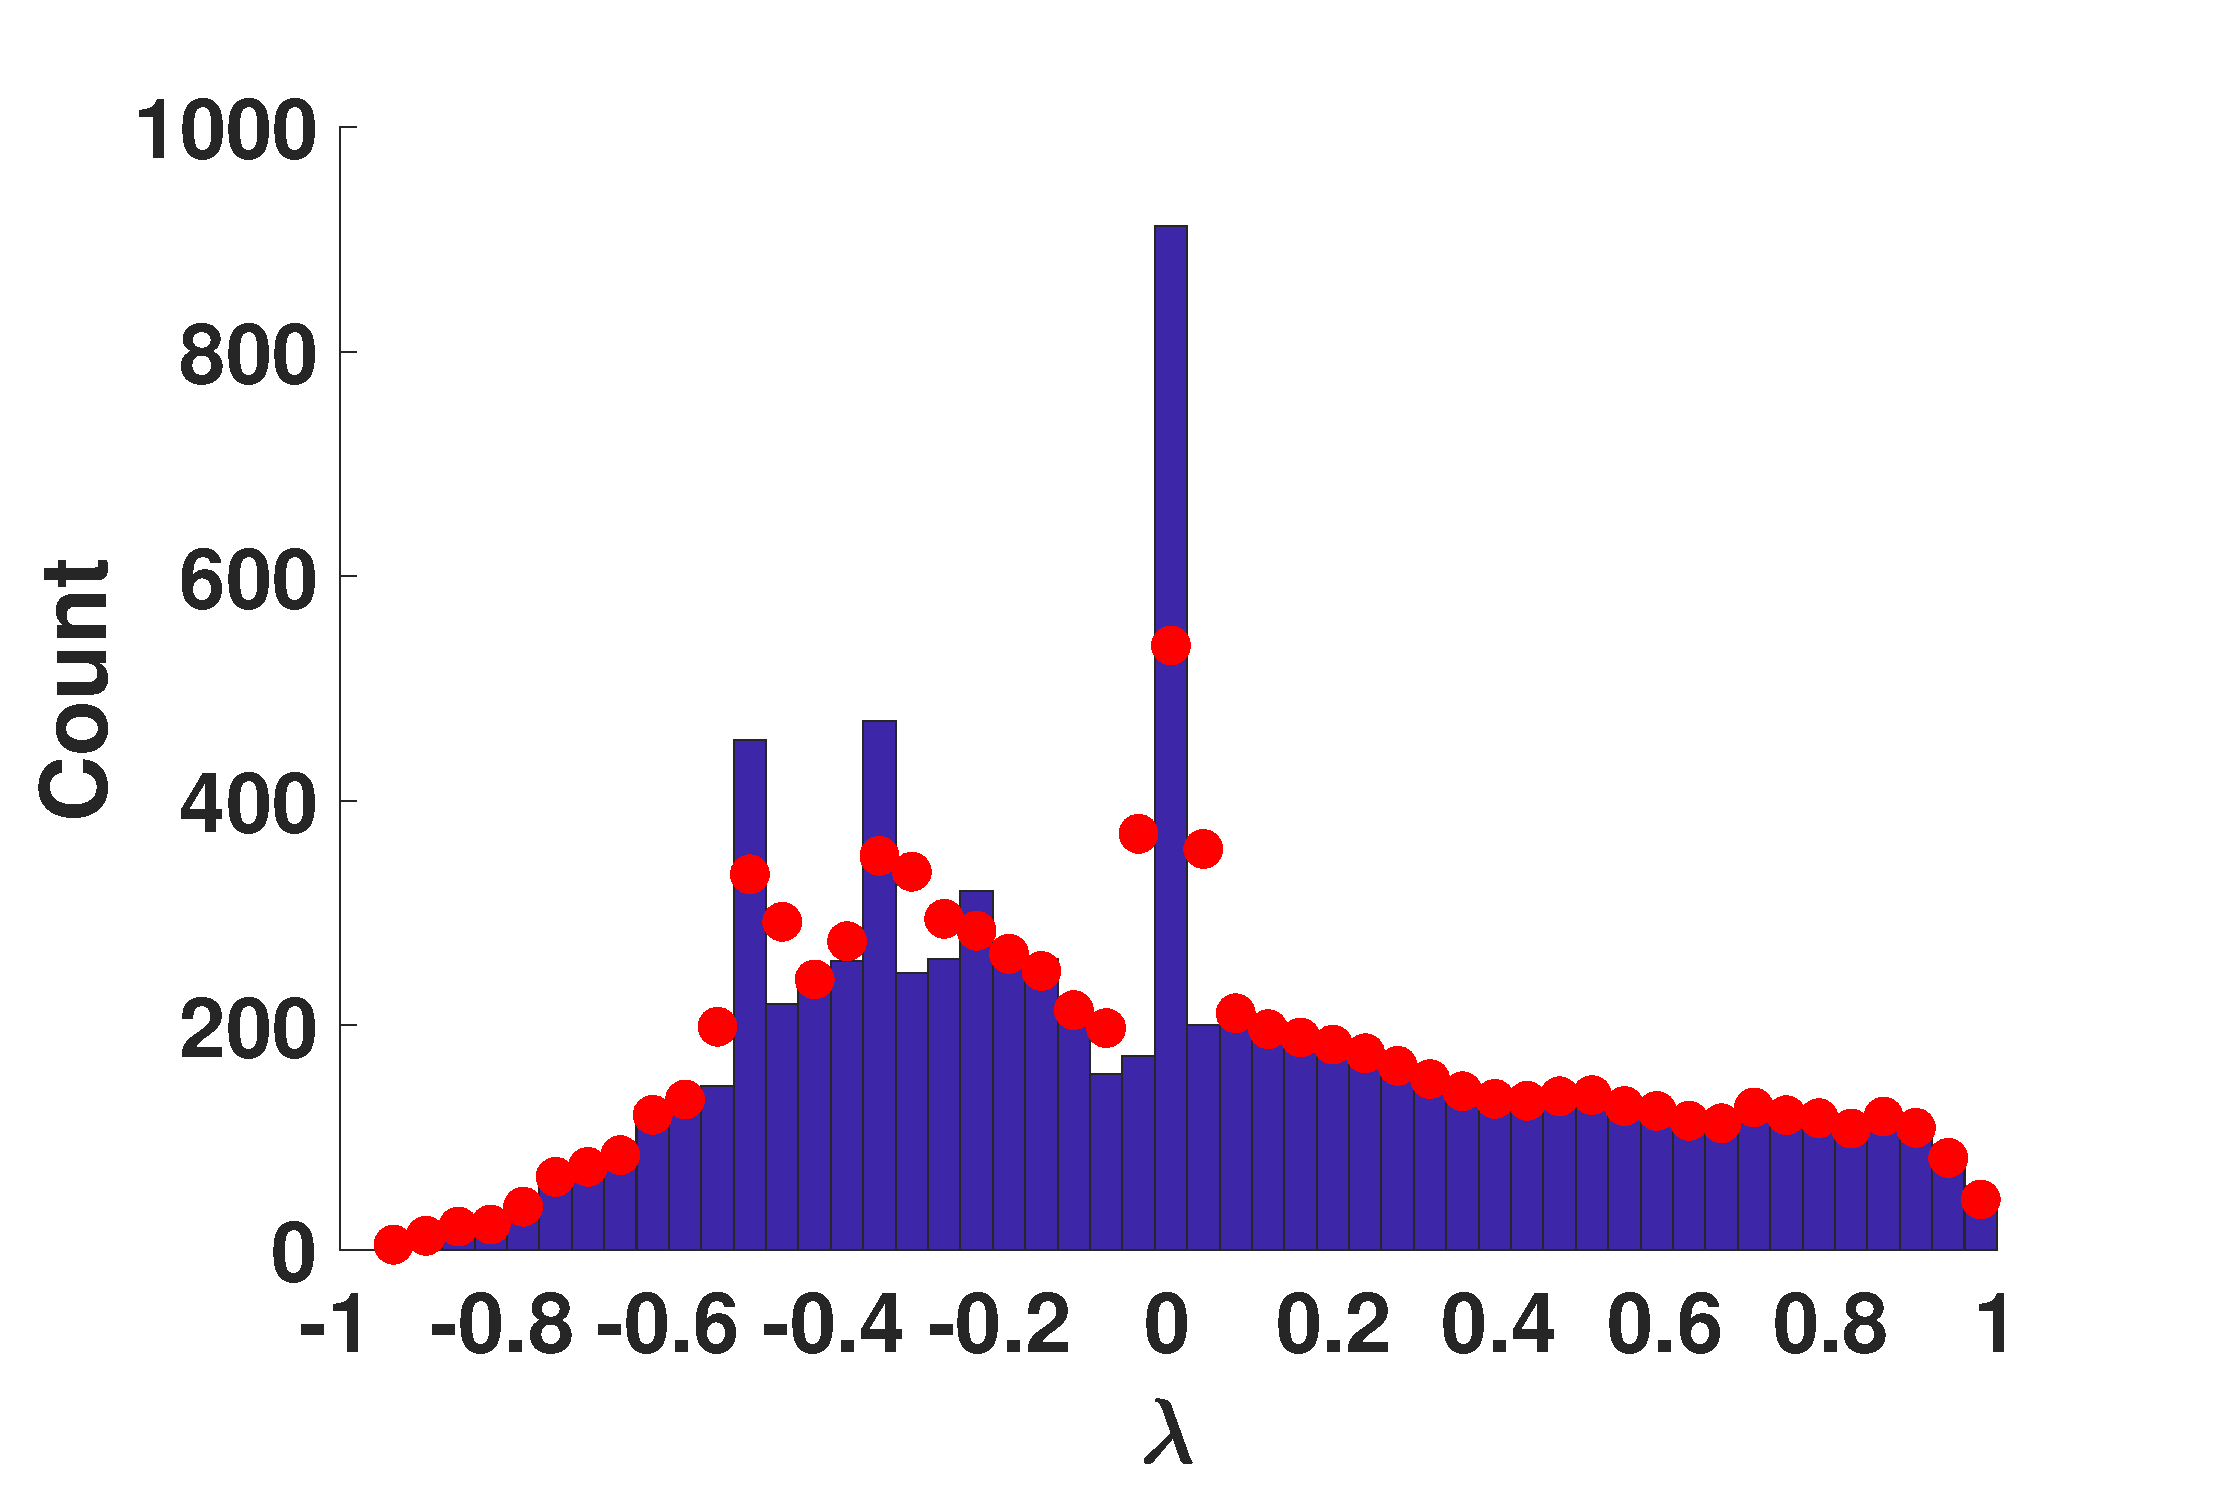
\includegraphics[width=\textwidth,trim = .3cm 0.5cm 3.2cm 1.3cm,clip]
    {./ndos/pics/hepth_nofilter}
    \caption{No Filter}\label{fig:hepth_0filt}
  \end{subfigure}
  %
  \begin{subfigure}{0.47\textwidth}
    \centering
    \captionsetup{justification=centering}
    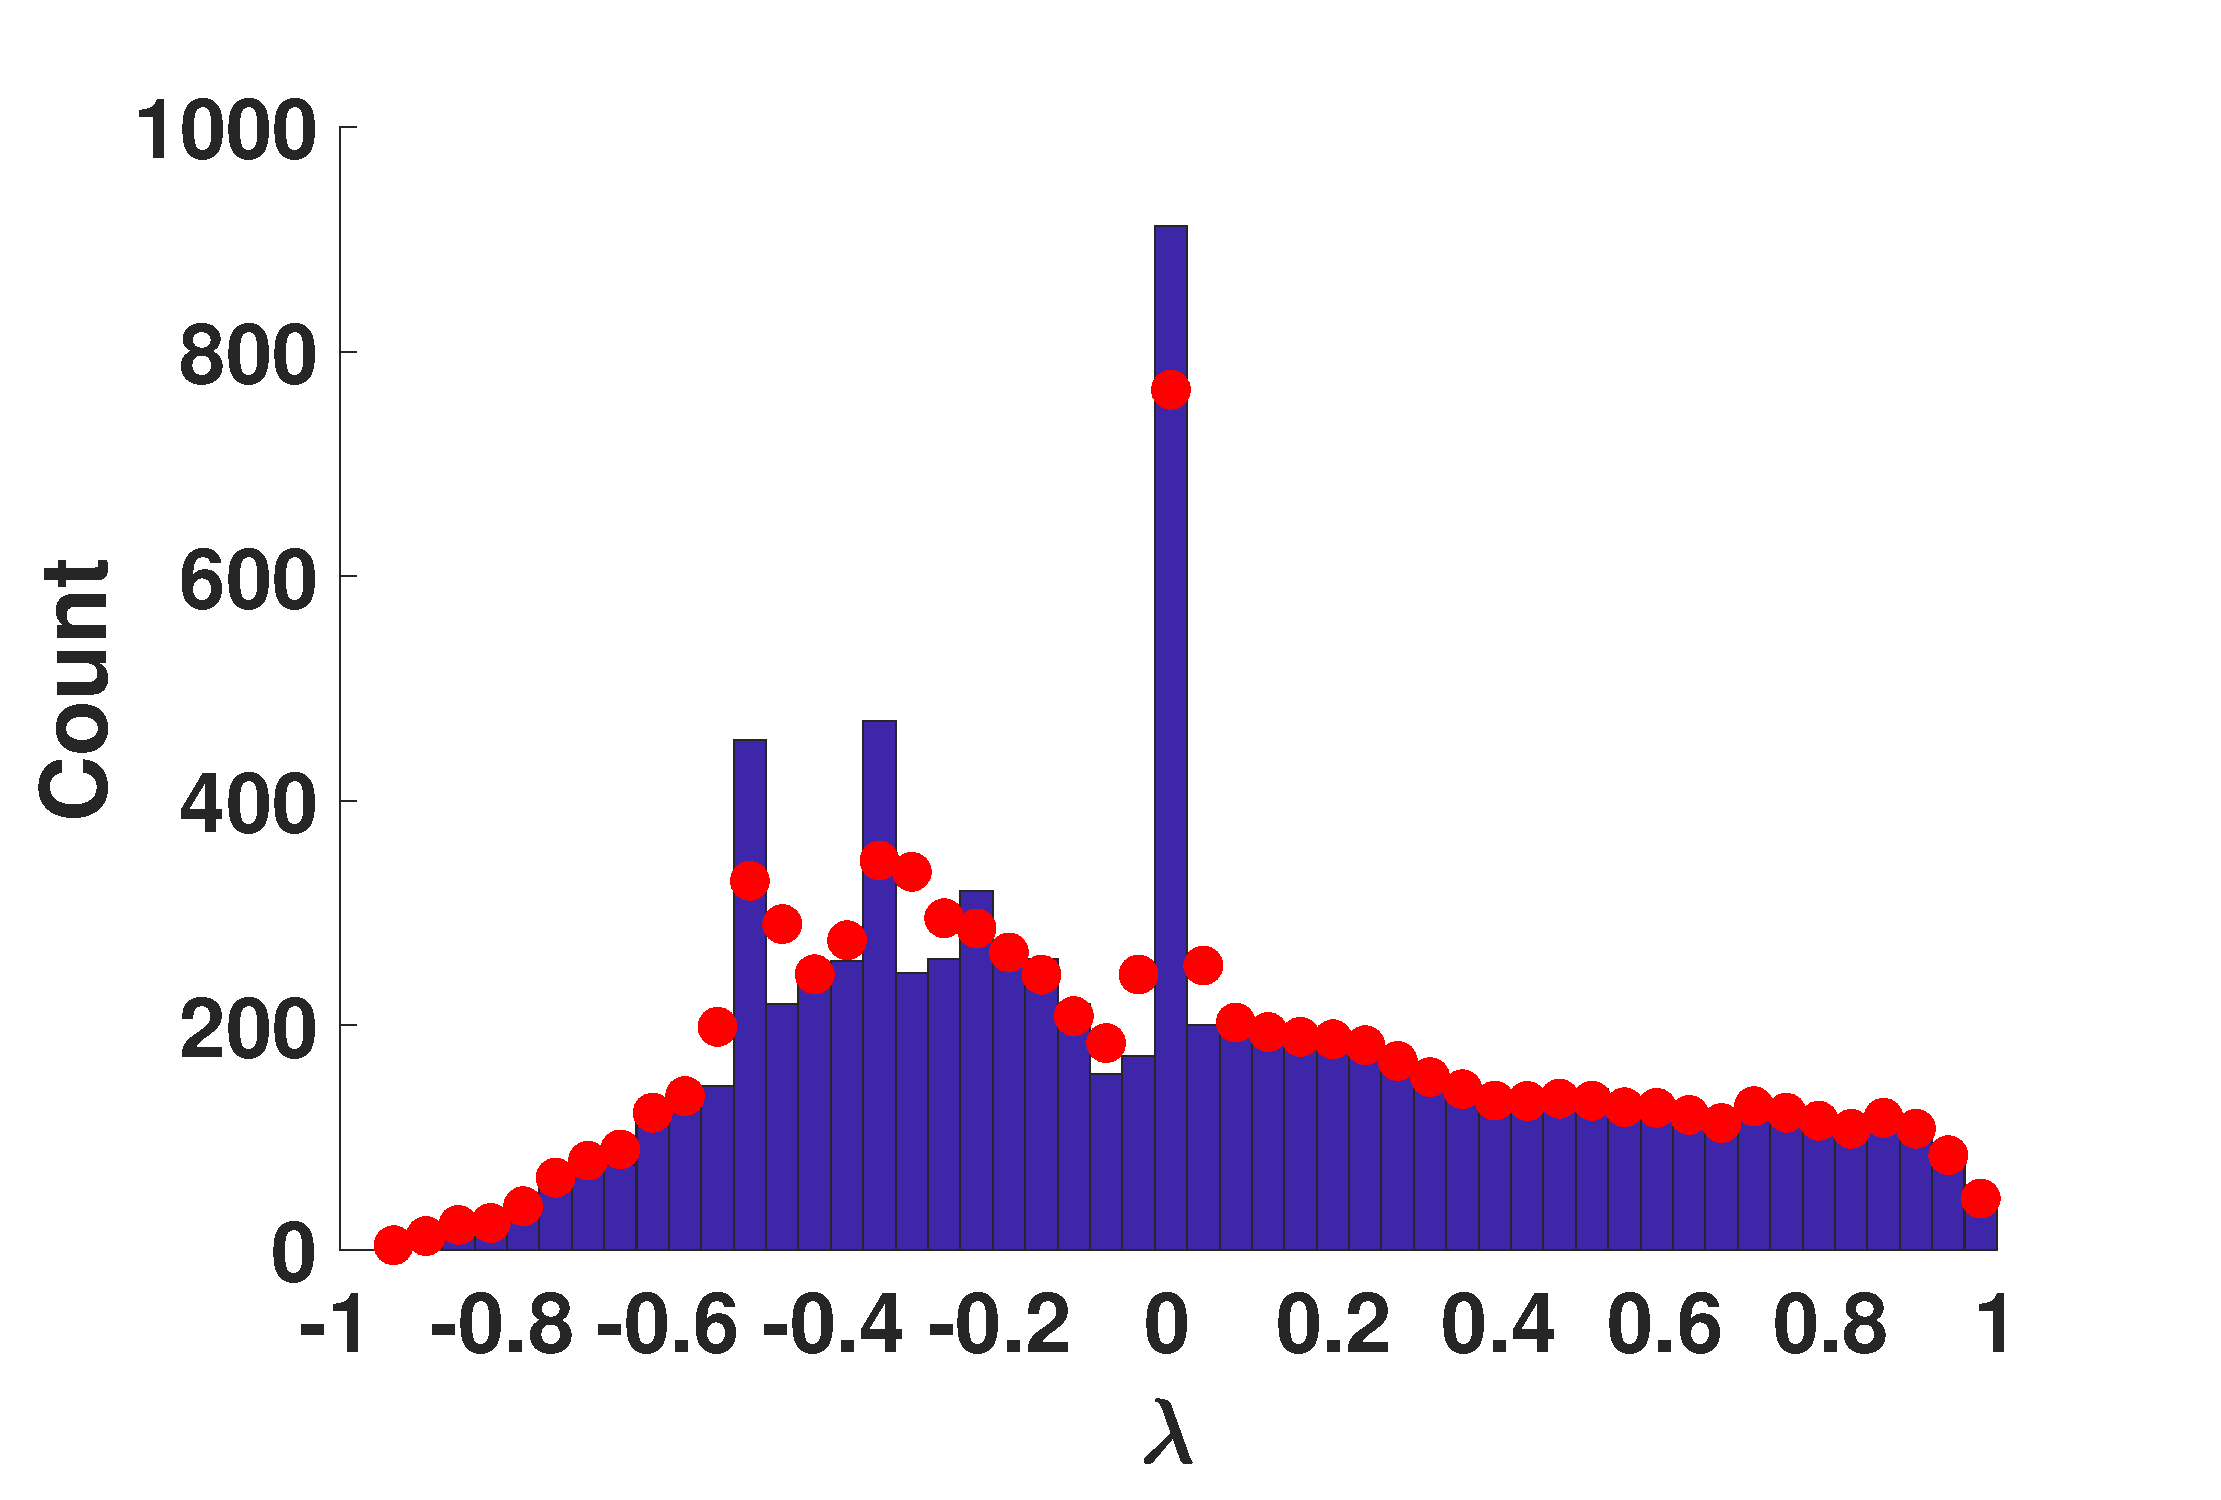
\includegraphics[width=\textwidth,trim = .3cm 0.5cm 3.2cm 1.3cm,clip]
    {./ndos/pics/hepth_onefilter}
    \caption{Filter at $\lambda=0$}\label{fig:hepth_1filt}
  \end{subfigure}
  %
  \begin{subfigure}{0.47\textwidth}
    \centering
    \captionsetup{justification=centering}
    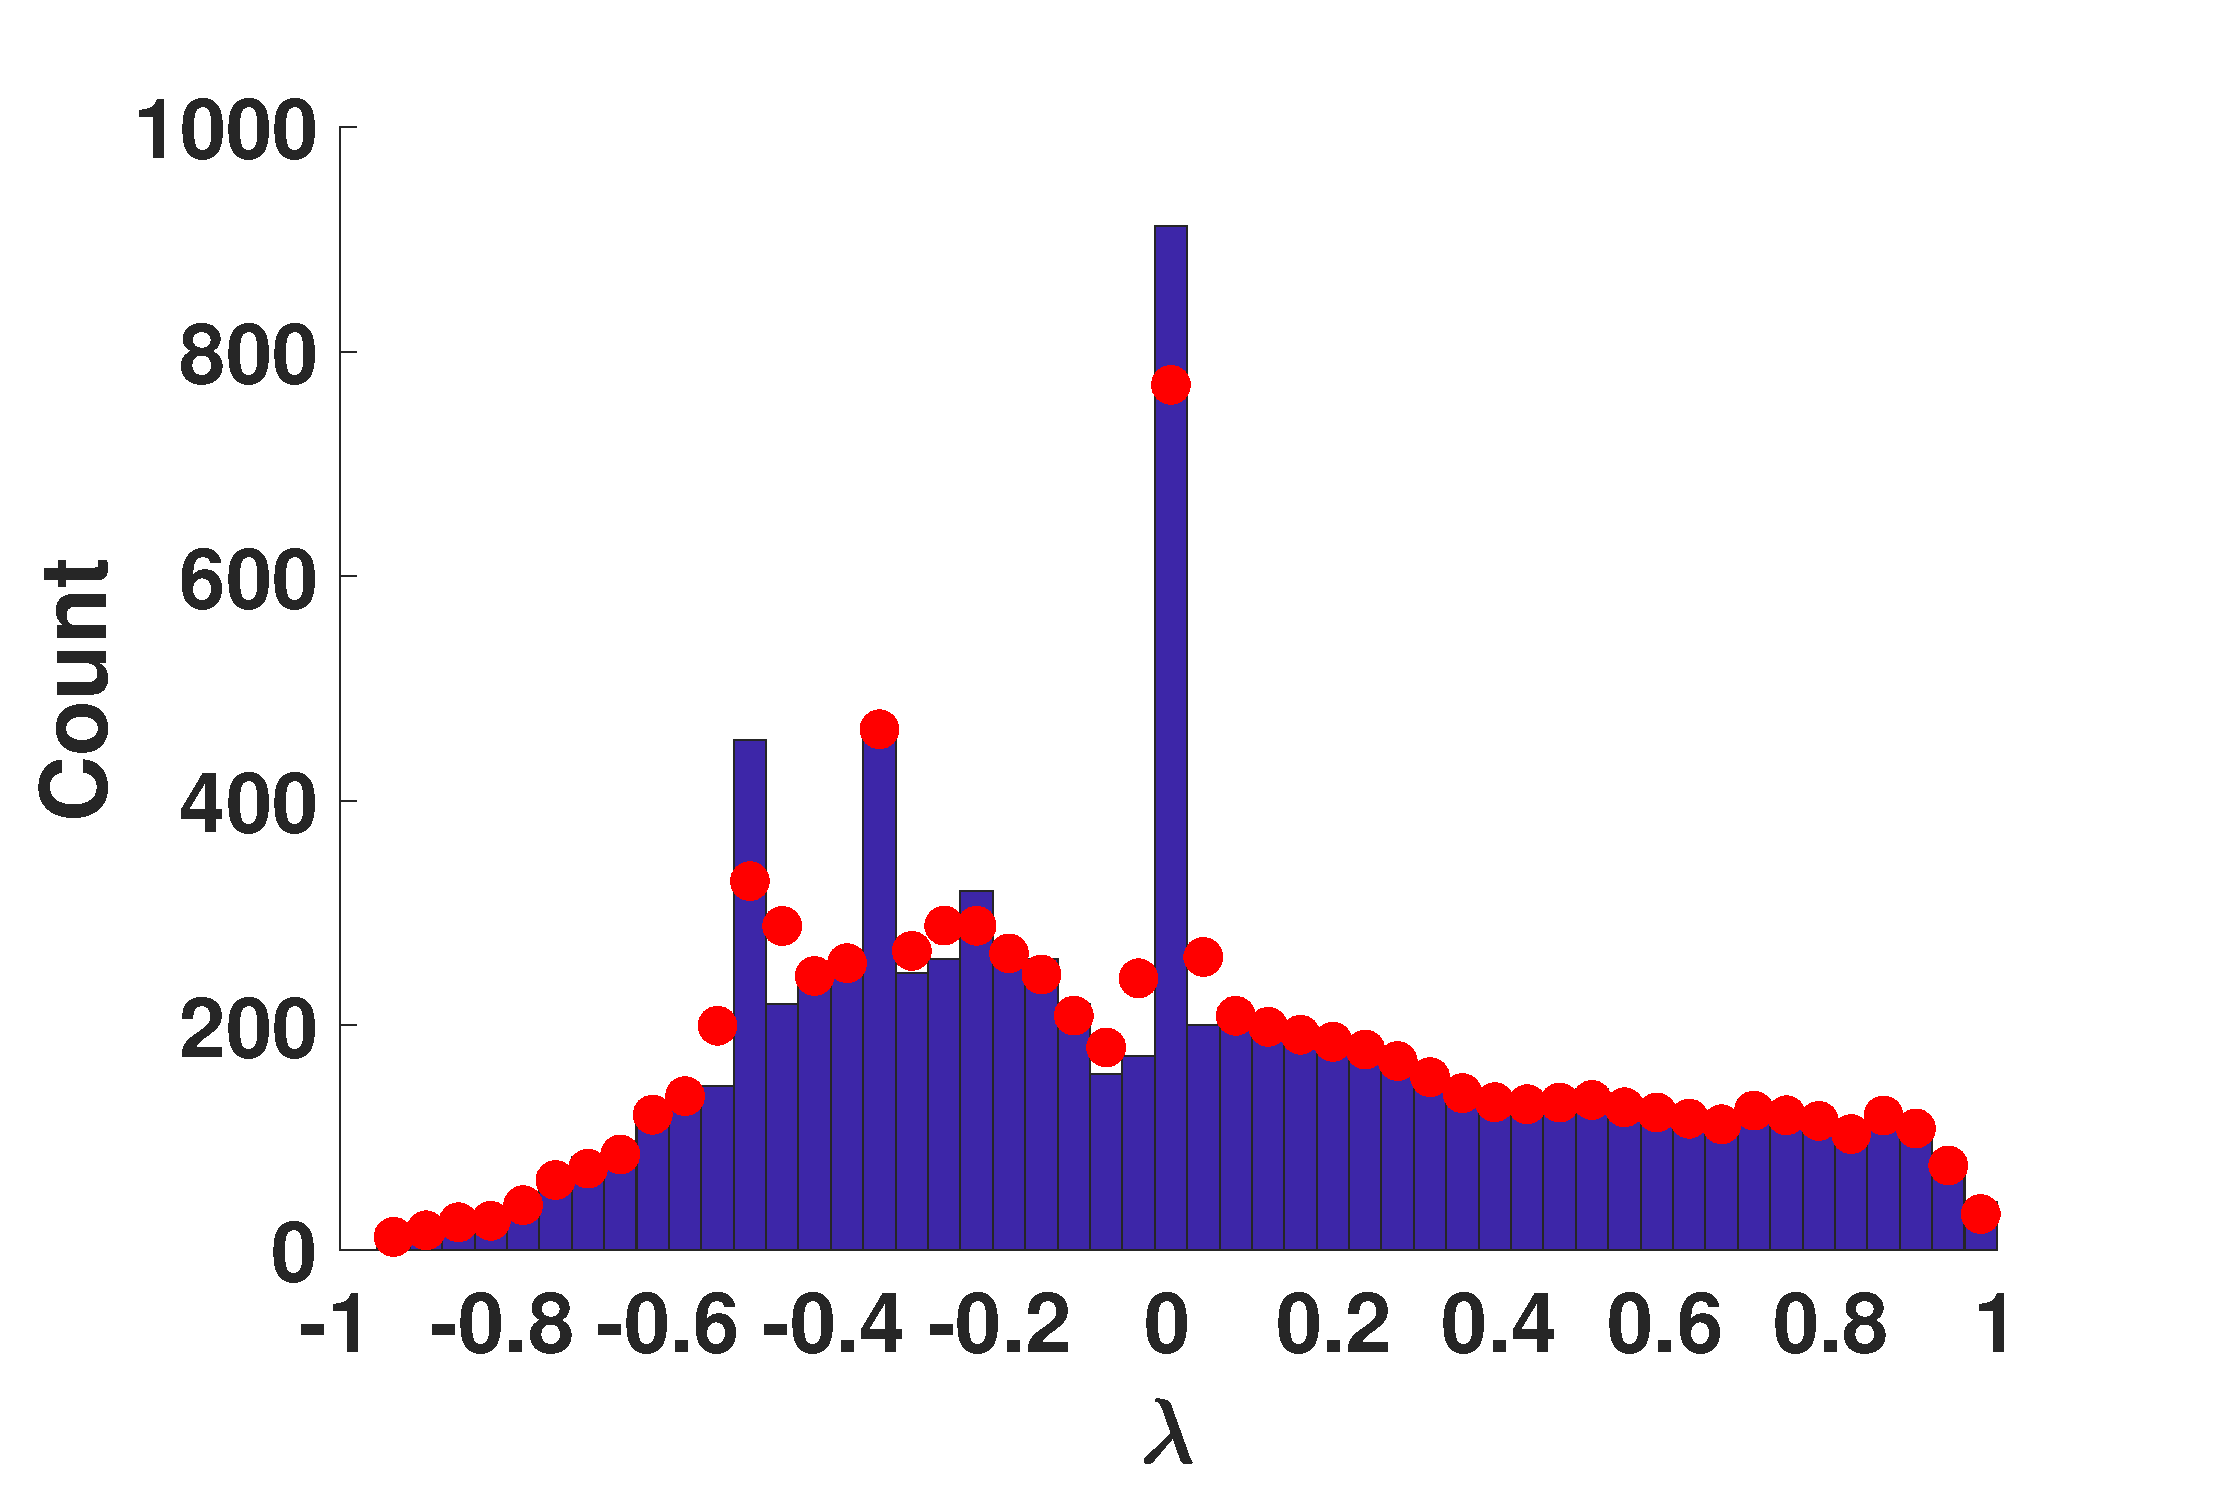
\includegraphics[width=\textwidth,trim = .3cm 0.5cm 3.2cm 1.3cm,clip]
    {./ndos/pics/hepth_twofilter}
    \caption{Filter at $\lambda=-1/3$}\label{fig:hepth_2filt}
  \end{subfigure}
  %
  \begin{subfigure}{0.47\textwidth}
    \centering
    \captionsetup{justification=centering}
    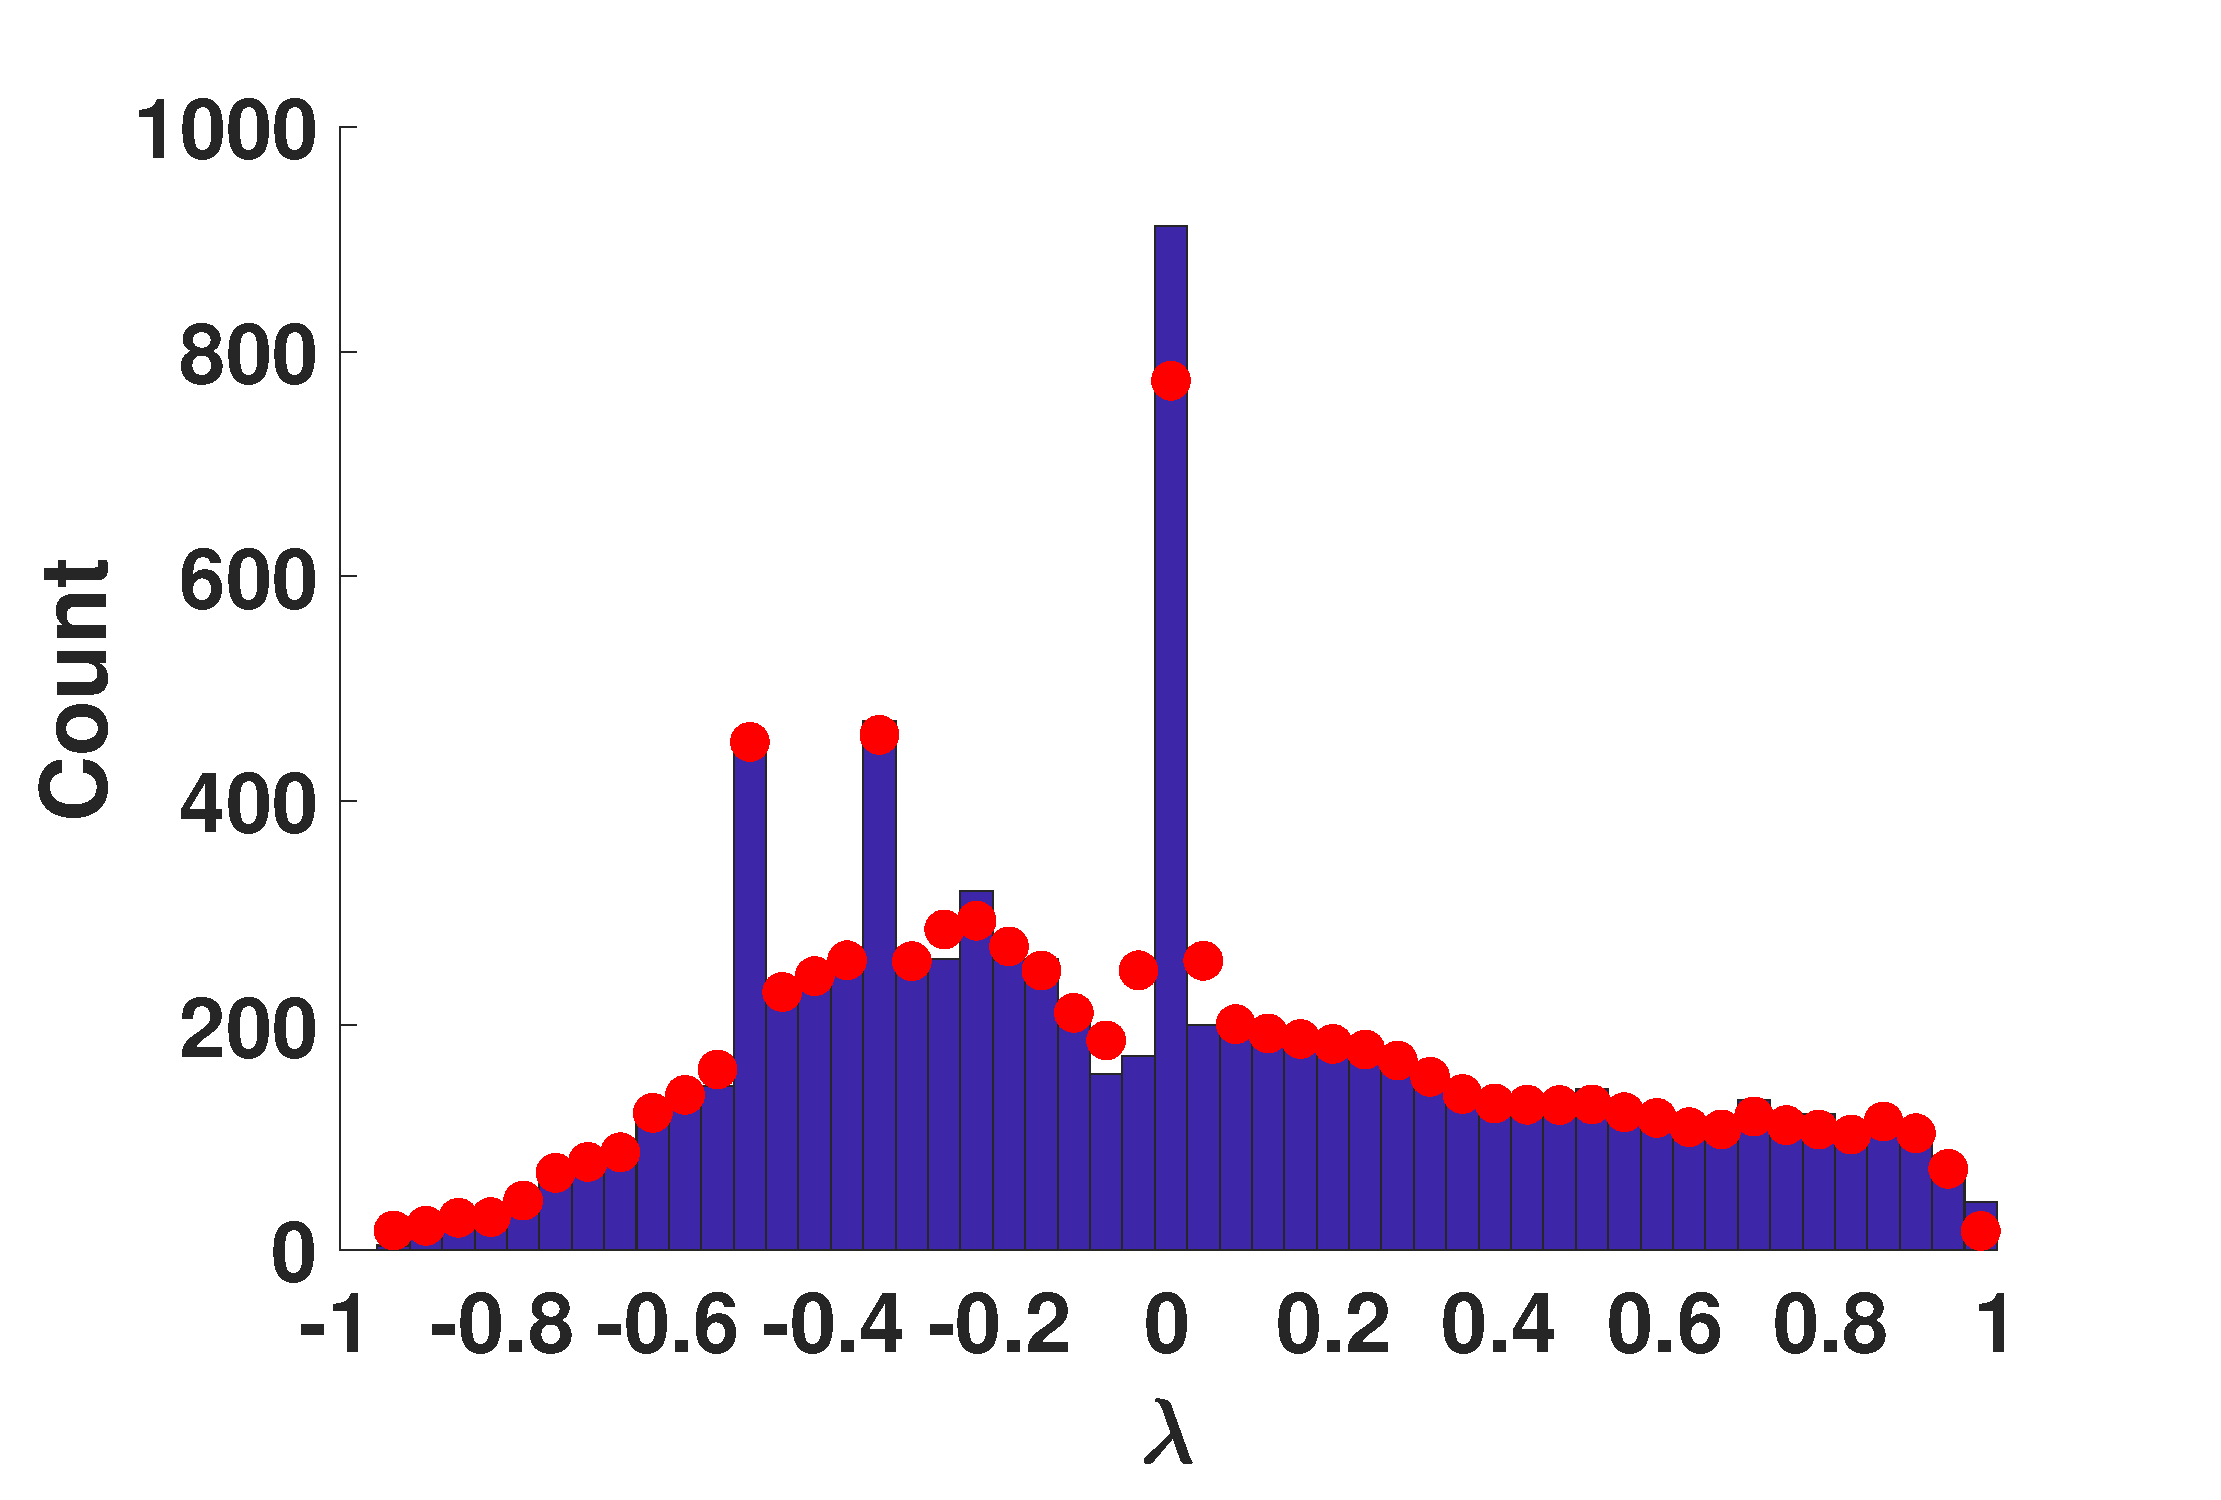
\includegraphics[width=\textwidth,trim = .3cm 0.5cm 3.2cm 1.3cm,clip]
    {./ndos/pics/hepth_threefilter}
    \caption{Filter at $\lambda=-1/2$}\label{fig:hepth_3filt}
  \end{subfigure}
  %
  \begin{subfigure}{0.47\textwidth}
    \centering
    \captionsetup{justification=centering}
    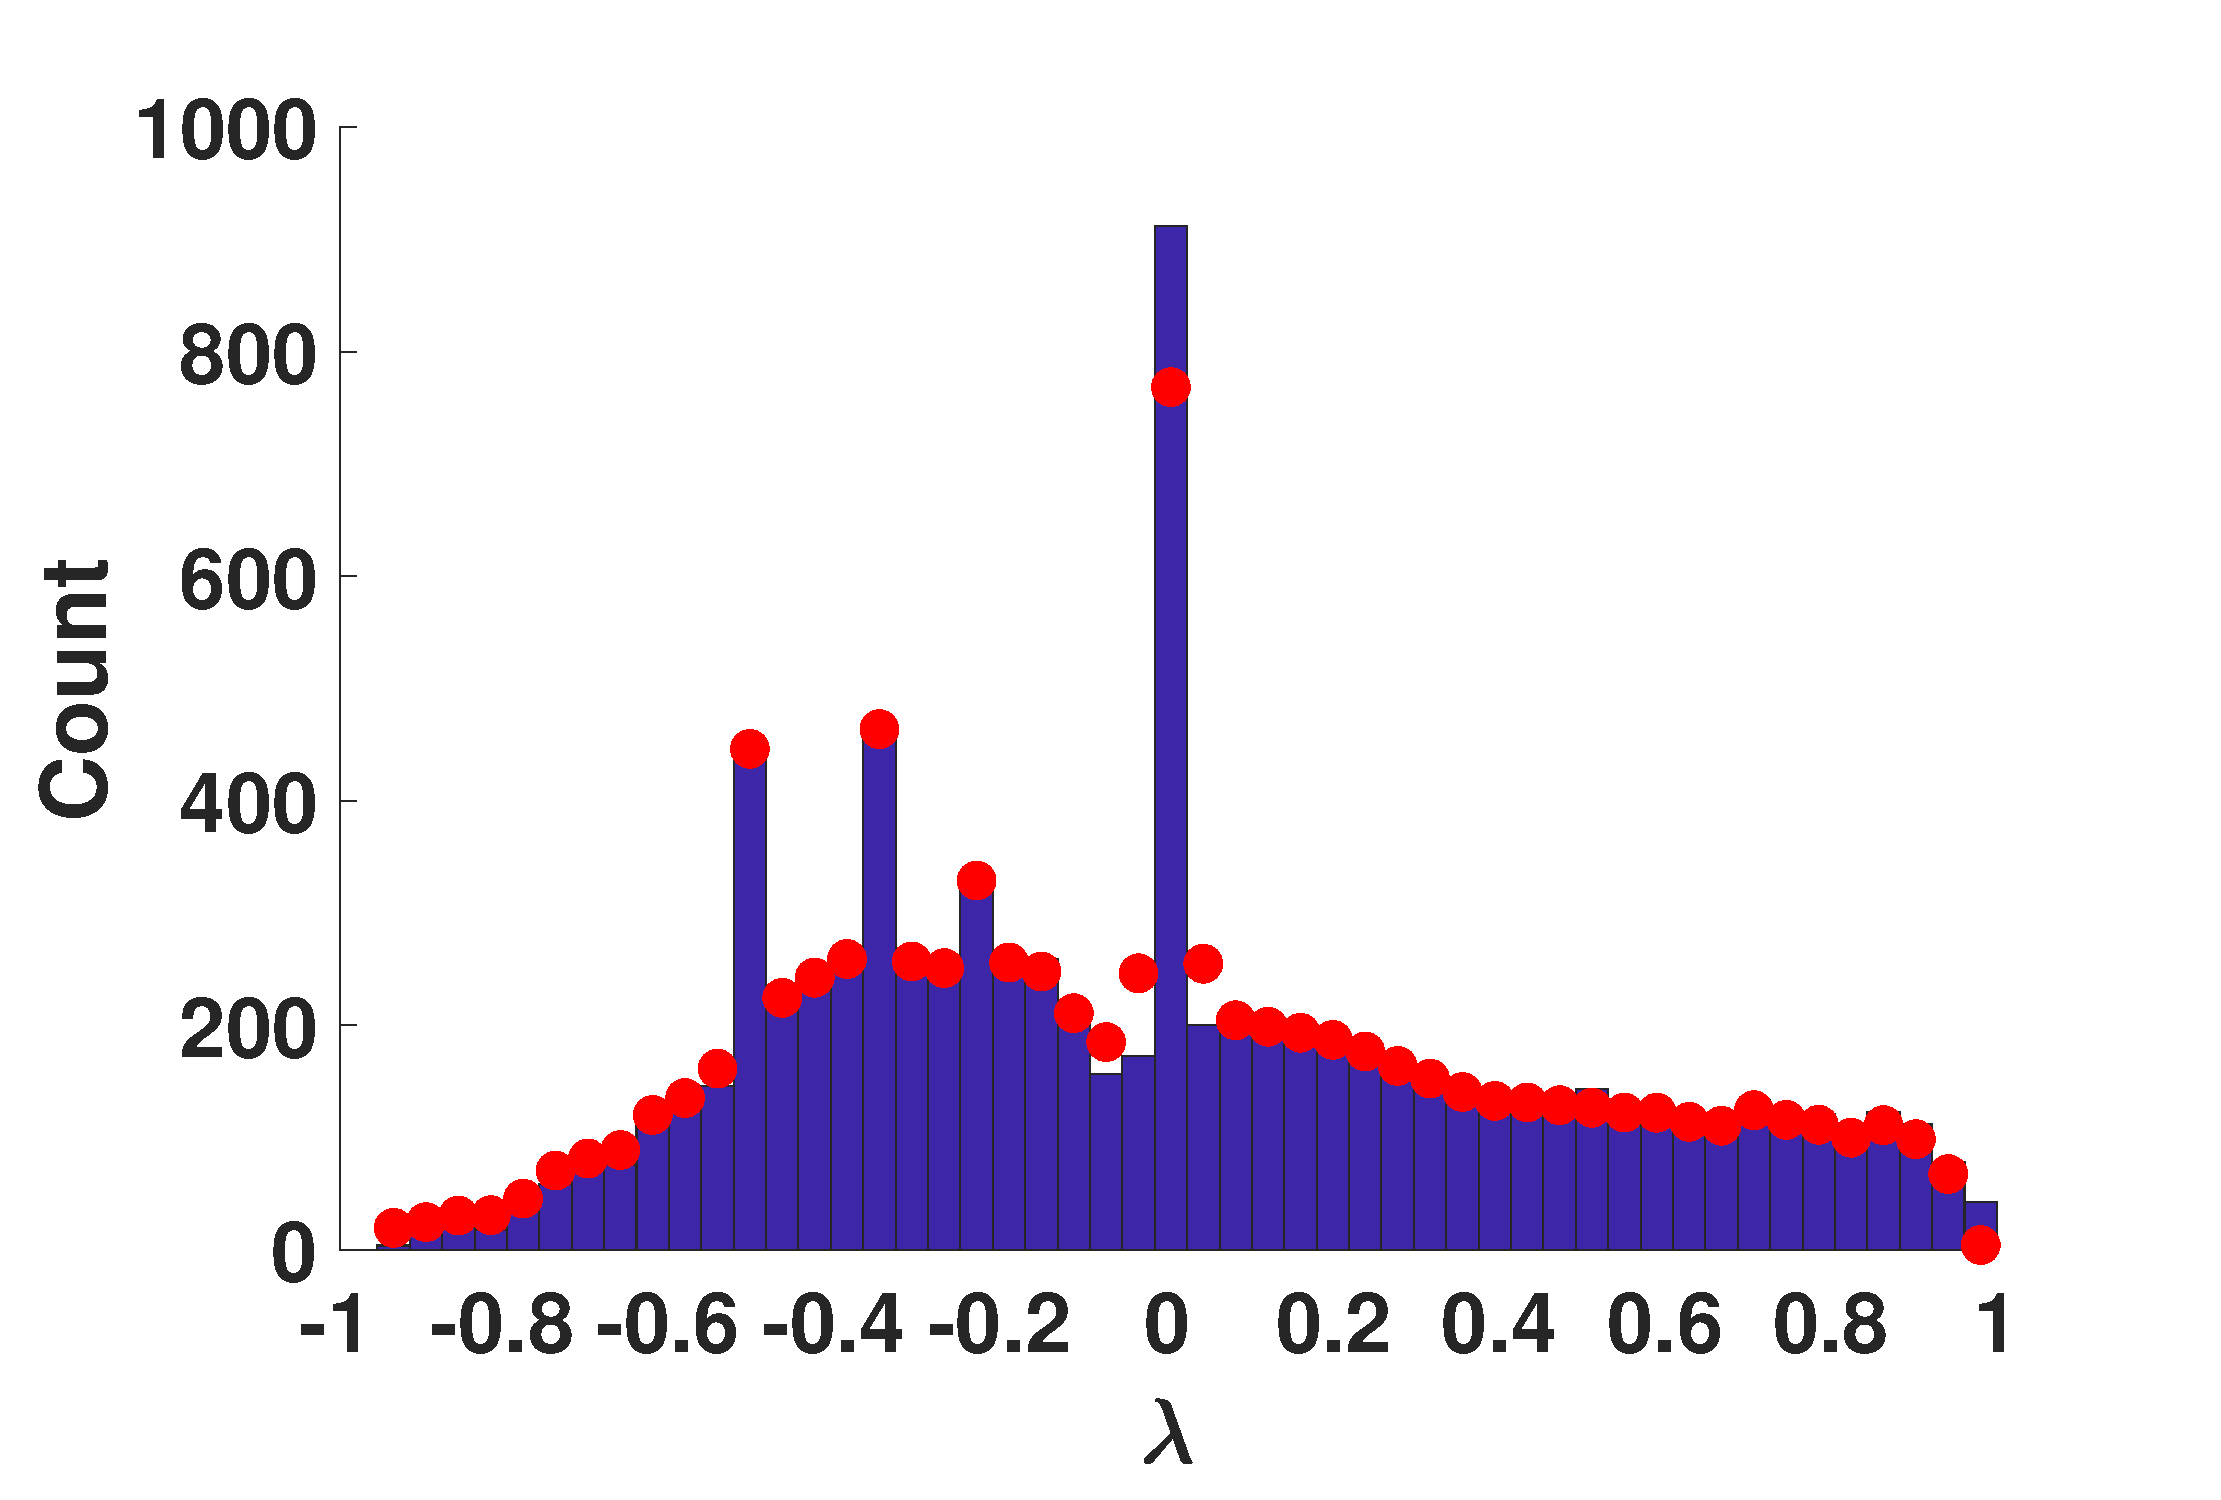
\includegraphics[width=\textwidth,trim = .3cm 0.5cm 3.2cm 1.3cm,clip]
    {./ndos/pics/hepth_fourfilter}
    \caption{Filter at $\lambda=-1/4$}\label{fig:hepth_4filt}
  \end{subfigure}
  %
  \hspace{0.8cm}
  \begin{subfigure}{0.47\textwidth}
    \centering
    \captionsetup{justification=centering}
    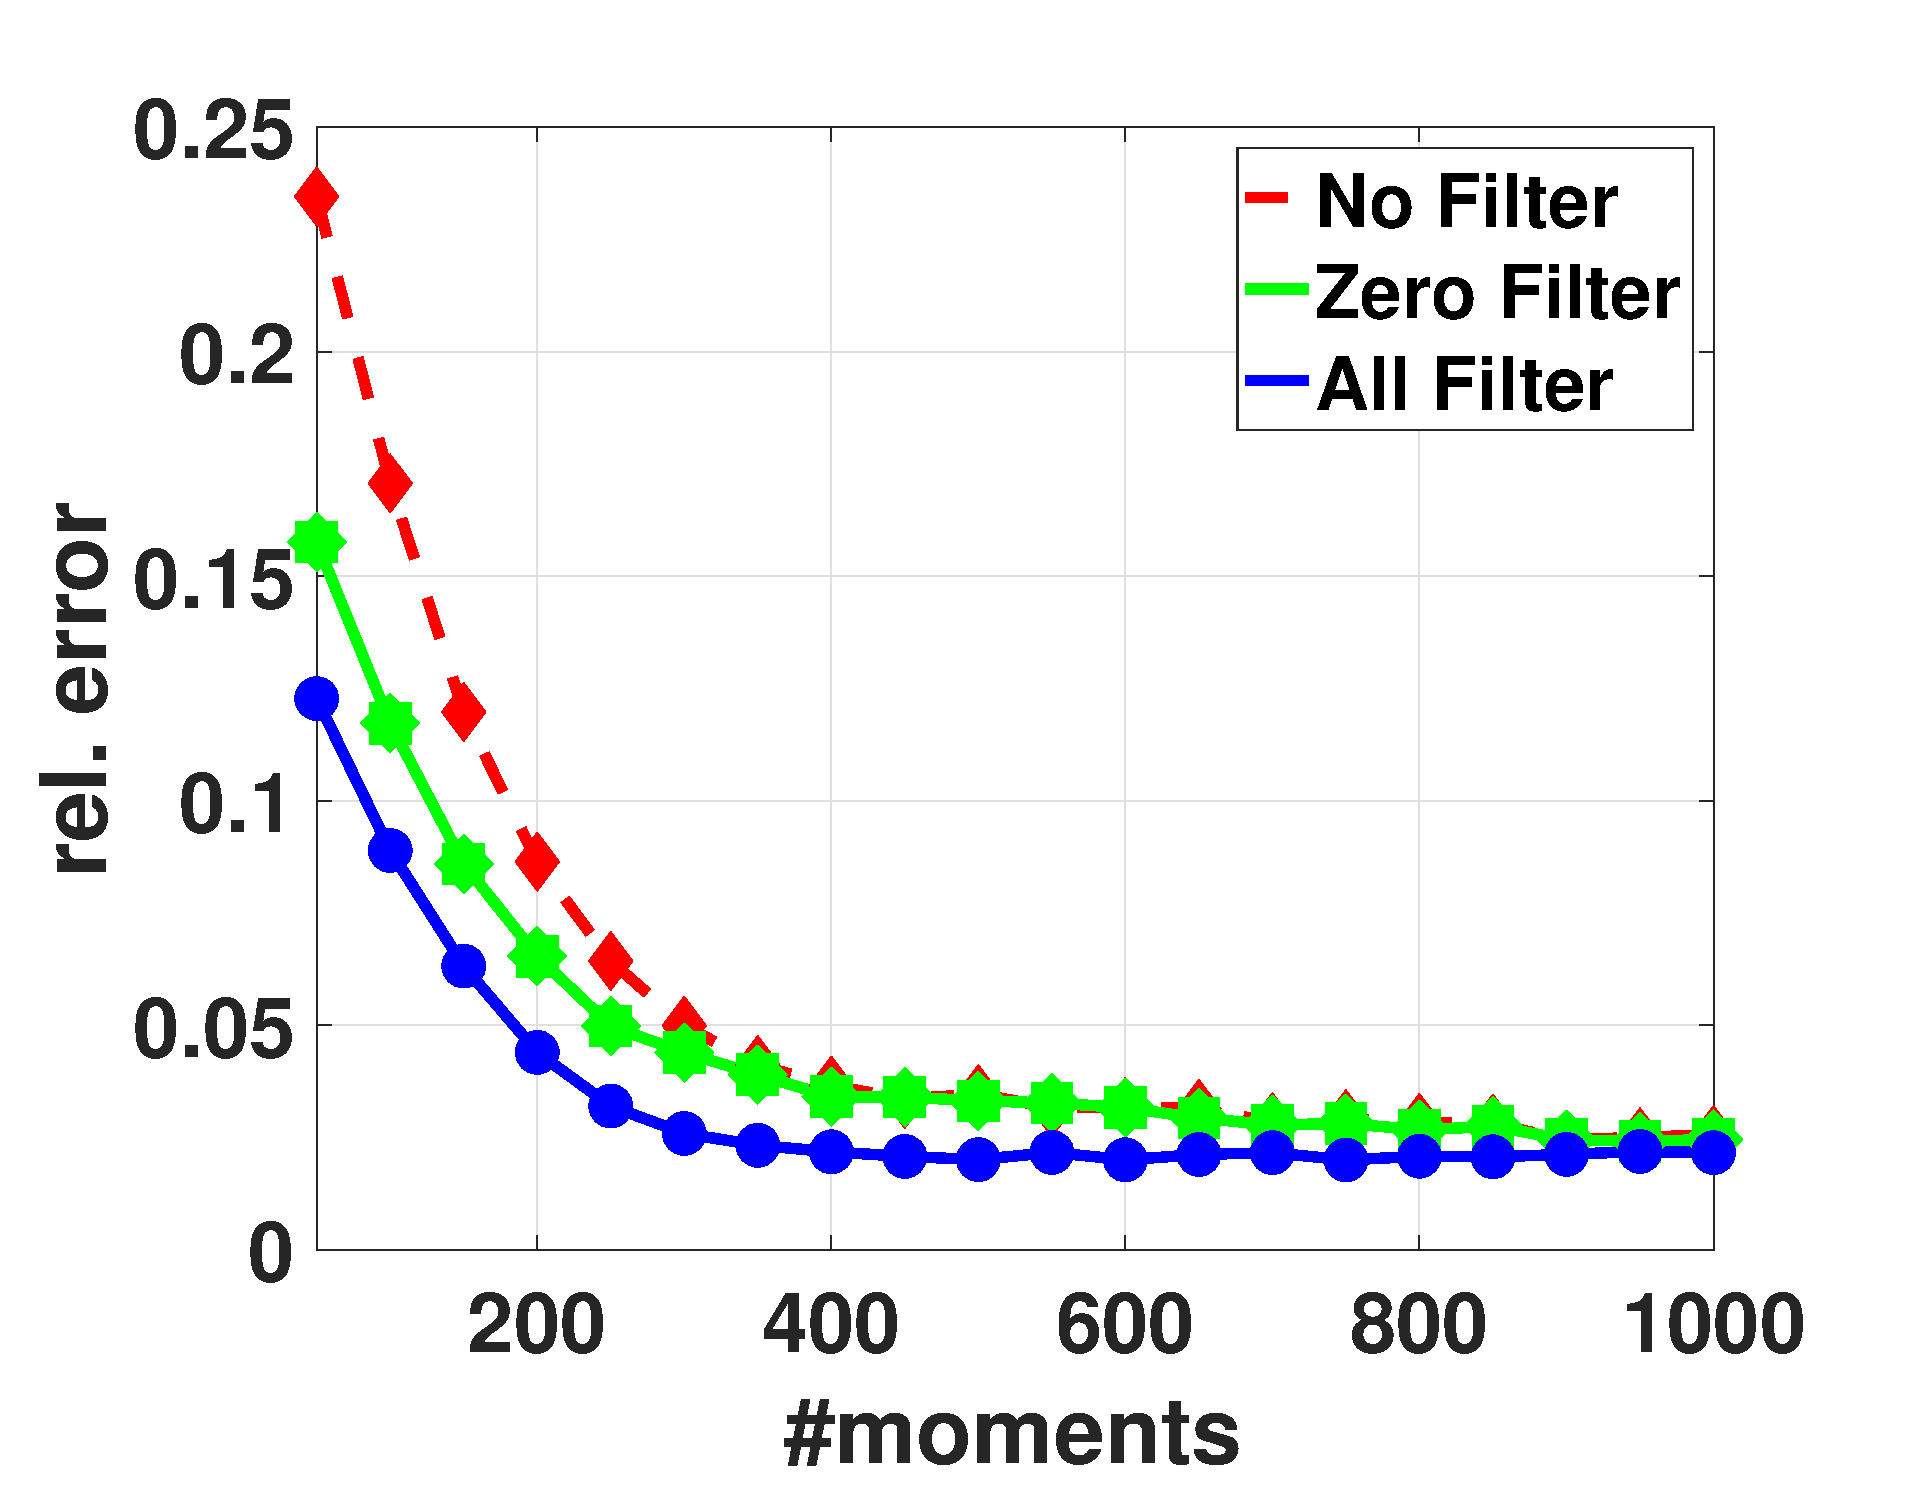
\includegraphics[width=0.9\textwidth,trim = .3cm 0cm 1.5cm 1.3cm,clip]
    {./ndos/pics/filter_error}
    \caption{Relative Error}\label{fig:hepth_error}
  \end{subfigure}
  \caption{The improvement in accuracy of the spectral histogram approximation
  on the normalized adjacency matrix for the High Energy Physics Theory (HepTh)
  Collaboration Network, as we sweep through spectrum and filter out motifs. The
  graph has $8,638$ nodes and $24,816$ edges. Blue bars are the real spectrum,
  and red points are the approximated heights. \cref{fig:hepth_0filt}-
  \ref{fig:hepth_4filt} use $100$ moments and $20$ probe vectors. \cref{fig:hepth_error} shows the relative $L_1$ error of the spectral
  histogram when using no filter, filter at $\lambda=0$, and all filters.}
  \label{fig:motif_filt}
\end{figure}